\chapter{Implementierung der Algorithmen}
\label{ch:implementierung}
\Autor{Sandra Schröder}\\\\
Im Rahmen des Projekts wurden zwei Algorithmen für die Skelettierung implementiert. Dies ist zum einen
die Skelettierung nach Thinning nach dem Algorithmus der in Abschnitt \ref{subsec:fastparallel} beschrieben wurde. Die Skelettierung mittels Distanztransformation wurde nach einer eigenen Idee entwickelt und
umgesetzt.\\
Die Skelettierung läuft in zwei Schritten ab. Erst wird der Spieler segmentiert. Man erhält als
Ergebnis ein Binärbild, welches im zweiten Schritt weiterverarbeitet wird, um ein Skelett zu extrahieren. 
Die Segmentierung des Spielers ist bei beiden Ansätzen identisch.
In diesem Kapitel wird die Umsetzung der Algorithmen anhand signifikanten Codeausschnitten der Implementierungen vorgestellt. Ein Überblick über die technische Umsetzung gibt einen Eindruck über die
verwendeten Programmiersprachen und Arbeitsumgebungen.
\section{Technische Umsetzung}
\label{sec:technische_umsetzung}
\Autor{Christopher Kroll}\\\\
F"ur die Implementierung wurden die bereitgestellten iMacs am Informatikum in Stellingen gew"ahlt. Der Vorteil war neben der Performanz die schon eingerichtete Arbeitsumgebung.\\
Um die Verbindung zu der Kinect herzustellen, wurde das quelloffene Framework libfreenect  der OpenKinect-Gruppe benutzt. Libfreenect bietet Treiber und Bibliotheken, um zum Beispiel die Bilder der Kamera anzuzeigen oder den eingebauten Motor zu steuern (siehe Abbildung \ref{fig:libfreenect}). \\
\begin{figure}
\centering
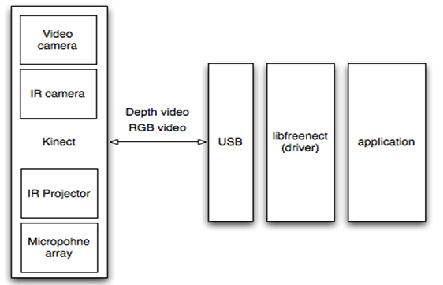
\includegraphics[width=0.7\linewidth]{./fig/libfreenect}
\caption{Libfreenect  \cite{libfreenect}}
\label{fig:libfreenect}
\end{figure}

Um die empfangenen Bilder verarbeiteten zu k"onnen wurde die Bibliothek OpenCV eingesetzt. Sie unterst"utzt unter anderem beim Speichern und Laden von Bildern und bei der Segmentierung. Wichtige Aufrufe von OpenCV-Funktionen werden im Folgenden an geeigneter Stelle erw"ahnt.\\
Eine weitere wichtige Bibliothek, die auch OpenCV benutzt, ist NumPy. Es ist eine Python-Erweiterung und wurde entwickelt, um Operationen bez"uglich mathematischen Funktionen und multidimensionalen Arrays effizienter zu gestalten \cite{numpy}. So wurde NumPy benutzt, um Arraywerte bei der Segmentierung logisch zu verkn"upfen (siehe Anhang \ref{anhang:segmentierung}). \\ \\ 
Der Gro"steil der Programmierung erfolgte in der Sprache Python. Hierbei handelt es sich um eine leicht zu erlernende Interpretersprache. Allerdings traten im Laufe des Projektes Performanzprobleme bei der Implementierung des Thinning-Algorithmus auf. 
 Aus diesem Grund wurde "uber einen Python-Wrapper der in C++ implementierte Algorithmus eingebaut. N"aheres dazu wird in Kapitel \ref{implThinning} beschrieben.

Als Entwicklungsumgebung wurde Spyder f"ur die Python-Programmierung und Apples Xcode f"ur die C++-Programmierung benutzt.

\section{Spielersegmentierung}
\label{segmentierung}
\Autor{Sandra Schröder}\\\\
Es wird anhand der Tiefeninformation segmentiert, die die Kinect liefert. Somit kann der Spieler in einfacher Weise vom Hintergrund und von anderen Objekten, die nicht skelettiert werden sollen, getrennt werden. Der Open-Source-Treiber für die Kinect - \emph{Freenect} - bietet Funktionen für den Zugriff auf die
Tiefenwerte. Die Funktion \texttt{pretty\_depth} des Moduls
\texttt{frame\_convert} normiert die Tiefenwerte auf das 
Intervall $[0,...,255]$. 
\lstset{
caption={Tiefenwerte zurückgeben}
\label{lst:getdepth}
}
\lstinputlisting{./listing/getdepth.py}
Um nicht für jeden einzelnen Pixel die Bedingung zu überprüfen, ob er den Schwellwert für die Segmentierung überschreitet beziehungsweise unterschreitet, wird die effiziente Numpy-Funktion \texttt{logical\_and} benutzt, die global auf dem Bild arbeitet und für das gesamte Bild die Schwellwertbedingung prüft. Eine pixelweise Überprüfung wäre mit Python eine ineffiziente Lösung.\\ Für den Schwellwert werden zwei 
Werte definiert, um ein Intervall festzulegen, in dem sich das Objekt befinden darf. In Listing \ref{lst:spielersegmentierung} legen die Variablen \texttt{current\_depth} und \texttt{threshold} das Intervall fest. 
\lstset{
caption={Spielersegmentierung in Python}
\label{lst:spielersegmentierung}
}
\lstinputlisting{./listing/player_segmentation.py}
Da die Funktion auf Numpy-Arrays arbeitet, muss das Bildobjekt zuvor in ein Array umgewandelt werden. 
Es wurden vorgefertigte Funktionen von OpenCV benutzt, die diese Konvertierung vornehmen. 
\section{Skelettierung mittels Thinning} 
\label{implThinning}
\Autor{Christopher Kroll} \\ \\
Da man sich schon durch den Seminarteil mit dem Algorithmus 'A Fast Parallel Algorithm for Thinning Digital Patterns' besch"aftigte, fiel die Wahl des Thinning-Algorithmus zun"achst auf diesen. \\
Der Algorithmus arbeitet mit Bin"arbildern, also alle Objektpixel sind auf 1, bzw. 255 gesetzt und alle Hintergrundpixel auf 0. Die in Kapitel \ref{segmentierung} vorgestellte Spieler-Segmentierung lieferte jedoch anfangs nur ein Grauwertbild. So war nun der erste Schritt dieses Bild in ein Bin"arbild umzuwandeln. Die Idee war das zweidimensionale Grauwertbildarray mit zwei Schleifen zu durchlaufen und jeden Wert, der gr"o"ser als 128 ist auf 255 zu setzen. Jeder Wert der kleiner oder gleich 128 ist, wird auf 0 gesetzt (siehe Listing \ref{lst:grayscaleToBinary}). 
\lstset{
caption={Binarisierung des Grauwertbildes.}
\label{lst:grayscaleToBinary}
}
\lstinputlisting{./listing/grayscaleToBinary.py}
So erhalten wir ein Array, das nur aus den Werten 0 und 255 besteht. Das Problem dabei war allerdings die nicht ausreichende Leistungsf"ahigkeit von Python. Schon bei diesen zwei ineinander verschachtelten Schleifen bestand keine Echtzeitf"ahigkeit mehr. Ohne auch nur den iterativen - und somit rechenintensiven - Thinning-Algorithmus eingesetzt zu haben stockte das Ergebnisbild zu stark. Python ist zwar "ahnlich schnell wie PHP, Perl oder Smalltalk, kann in Sachen Geschwindigkeit mit kompilierten Sprachen jedoch nicht mithalten \cite{python}. \\Aus diesem Grund musste eine Alternative zu Python gefunden werden. Die Wahl fiel auf die leistungsst"arkere Compilersprache C++. \\ \\
Nun sollten jedoch nicht zwei unterschiedliche Programme entstehen - Distanztransformation mit Python und Thinning mit C++ und die Spieler-Segmentierung in Python sollte auch f"ur die Thinning-Skelettierung benutzt werden. Die L"osung war die M"oglichkeit der Anbindung von Python an eine andere Programmiersprache, in diesem Fall C++. So wurde der in Kapitel \ref{ch:Skelettierung} vorgestellte Thinning-Algorithmus in C++ geschrieben und mit einem Makefile kompiliert. Der kompilierte Code wurde nun mit einem Wrapper eingebunden. Die Python-Datei pythonWrapper.py l"adt daf"ur die vom Makefile erstellte Bibliothek, um auf die kompilierten Daten zuzugreifen (Listing \ref{lst:loadlib}) .
\lstset{
caption={Laden der Wrapper-Bibliothek.}
\label{lst:loadlib}
}
\lstinputlisting{./listing/loadlib.py}
Die C++-Funktion kann nun mit Python aufgerufen werden (Listing \ref{lst:callC}).
\lstset{
caption={Aufruf der C++-Funktion.}
\label{lst:callC}
}
\lstinputlisting{./listing/callC.py}

Da nun mit dem 'A Fast Parallel Algorithm for Thinning Digital Patterns'-Algorithmus trotz mehrst"undiger Fehlersuche und Optimierung jedoch keine guten Ergebnisse erzielt werden konnten, wurde auf den verwandten Guo-Hall-Algorithmus zur"uckgegriffen. Auch er hat vier Kriterien, die zutreffen m"ussen, damit ein Pixel gel"oscht werden kann. Aufgrund der Pixelbenennung im 3x3-Pixel-Fenster aus Abbildung 3.2 ergeben sich folgende Kriterien in der C++-Implementation: \\
\lstset{
caption={Guo-Hall-Kriterien in C++}
\label{lst:thinningImpl}
}
\lstinputlisting{./listing/thinningImpl.py}
Treffen die Kriterien in Zeile 7 zu, wird der Pixel in Zeile 8 zum L"oschen markiert.

\section{Skelettierung mittels Distanztransformation}
\label{sec:impl_distanztrans}
\Autor{Sandra Schröder}\\\\
Der theoretische Ablauf der Skelettierung wurde bereits im Kapitel \ref{ch:Skelettierung} beschrieben. Zur
Rekapitulation werden die Schritte kurz aufgezählt. \\
Die Skelettierung anhand der Distanztransformation läuft folgendermaßen ab:
\begin{itemize}
\item Bestimmen der Distanztransformation des Binärbildes
\item Berechne den Gradientenbetrag auf der Distance Map und führe die Segmentierung auf dem Gradientenbetragsbild aus.
\item Differenz zwischen dem Gradientenbild und der Distance Map bilden
\end{itemize}
Die Distance Map kann mit einer Funktion aus der Bildverarbeitungsbibliothek \emph{OpenCV} einfach berechnet
werden. Die Funktion (Listing \ref{lst:disttransform}) erwartet als Eingabe das Originalbild (\texttt{img}) und ein Bild (\texttt{dist\_img}), um
das Ergebnis speichern zu können (gleiche Größe und Dimension wie das Originalbild). Eine weitere Möglichkeit, die die Funktion bietet, ist die Angabe einer Metrik, nach der der Abstand eines Pixels zum
Hintergrund bestimmt wird. Es wurde die euklidische Metrik benutzt.
\lstset{
caption={Berechnen der Distance Map des Binärbildes des Spielers.}
\label{lst:disttransform}
}
\lstinputlisting{./listing/distancetransform.py}
Zur Bestimmung des Gradientenbetrages der Distance Map wurde die Numpy-Funktion \texttt{gaussian\_gradient\_magnitude} genutzt (Listing \ref{lst:gradient}). Die Funktion berechnet den Gradientenbetrag mit Ableitungen
der Gaussfunktion. Die Variable \texttt{sigma} ist die Standardabweichung 
des Gaussfilters. Das Ergebnis dieser Funktion wird in ein Bildobjekt
konvertiert und entsprechend festgelegter Schwellwerte (\texttt{lowerbound}, \texttt{upperbound}) segmentiert.
\lstset{
caption={Gradientenbetrag der Distance Map und Segmentierung des Gradientenbetragsbildes.}
\label{lst:gradient}
}
\lstinputlisting{./listing/gradient.py}
Zur Differenzbildung und endgültigen Berechnung des Distanzskelettes werden die Bildobjekte in Arrays umgewandelt. Diese Arrays können einfach voneinander abgezogen werden (Listing \ref{lst:difference}). 
\lstset{
caption={Differenz zwischen Distance Map und segmentiertem Gradientenbetrag}
\label{lst:difference}
}
\lstinputlisting{./listing/difference.py}
Bei der Implementierung wurden in keinem Fall Operationen ausgeführt, die auf einzelne Pixel zugreifen. Situationen, in denen
pixelweise Operationen durchgeführt werden könnten, wurden
umgangen, indem Arrayoperationen oder Funktionen aus der
OpenCV-Bibliothek benutzt wurden. Ein pixelweiser Zugriff
könnte bei einer Interpretersprache wie Python zu einer sehr langsamen
Ausführung der Skelettberechnung führen.